\section{방법론}

Kronos는 금융 K-line 시퀀스를 이산 언어로 추상화하고, Figure~\ref{fig:overview}에 설명된 두 단계 프레임워크, 즉 \textbf{(1) K-line 토큰화}와 \textbf{(2) 자기회귀 사전학습}을 통해 이를 구현한다. 첫 번째 단계에서는 연속적인 다변량 K-line 시퀀스를 학습 가능한 코드북을 통해 대응되는 이산 토큰 시퀀스로 양자화하기 위해 특화된 Transformer 기반 tokenizer를 설계한다. 각 K-line 항목(OHLCVA)은 개별 인스턴스로 취급되어 이산 토큰으로 양자화된다. 각 토큰은 coarse-grained subtoken과 fine-grained subtoken으로 구성된다.
이 속성은 계층적 재구성 손실을 통해 강제되며, 이는 subtokens가 서로 다른 정보 수준을 모델링하도록 명시적으로 유도함으로써 coarse-to-fine 정보 계층을 형성한다.
두 번째 단계에서는 표준 next-token prediction 목적을 사용하여, 주어진 과거 문맥에 조건화된 각 미래 시점에서 두 subtoken 수준을 순차적으로 예측하도록 이러한 토큰화된 시퀀스에 대해 decoder-only Transformer를 자기회귀적으로 사전학습한다. 이 통합된 \emph{discretize-and-generate} 패러다임은 Kronos가 시장 동학의 고충실도 계층적 표현을 구축할 수 있게 하며, downstream 정량 분석을 위한 견고한 기반을 제공한다.

\subsection{K-line 토큰화}

Kronos의 첫 번째 단계는 OHLCVA 지표를 인코딩하는 $\mathbf{x}_{t}\in\mathbb{R}^{D}$로 이루어진 연속적인 $D$차원 K-line 시퀀스 $\mathbf{x} = (\mathbf{x}_{1}, \ldots, \mathbf{x}_{T})$를 대응되는 이산 토큰열로 변환한다. 이는 encoder $E_{\text{enc}}$, quantizer $Q$, decoder $E_{\text{dec}}$로 구성된 Transformer 기반 autoencoder(Figure~\ref{fig:tokenizer})를 사용하여 달성된다. 생성 모델링의 비디오 양자화 방법~\cite{van2017neural,yu2023language}에서 영감을 받아, 우리는 Binary Spherical Quantization (BSQ)~\cite{zhao2024image}, 즉 Look-up Free Quantization (LFQ)~\cite{yu2023language}의 변형을 이 과제에 맞게 적용한다.
이 선택의 근거는 Appendix~\ref{sec:discussion} (Q2)에서 논의한다.
BSQ는 연속 잠재 벡터 $\bm{\xi}_t$를 학습 가능한 초평면들의 집합에 투영함으로써 $k$-bit 이진 코드 $b_t \in \{-1,1\}^k$로 양자화한다. 풍부한 금융 패턴을 포착하기 위해 큰
bit 수 $k$(예: $k=20$)가 바람직하지만, 이는 크기가 $2^k$인 지수적으로 큰 vocabulary를 초래하여 이후 자기회귀 모델의 계산 비용과 파라미터 크기 측면에서 상당한 문제를 야기한다. 이를 완화하기 위해, 우리는 비디오 양자화 및 생성에 관한 최근 연구~\cite{yu2023language,wang2025bridging}를 따라 $k$-bit 코드를 $n$개의 subspace로 factorize한다. Appendix~\ref{sec:discussion} (Q3)에 자세히 설명된 파라미터 절감과 지연 비용 간의 trade-off에 근거하여, 우리는 $n=2$로 설정한다. 코드를 동일한 bit 길이 $k_c = k_f = k/2$를 갖는 coarse subtoken $b_{t}^{c}$와 fine subtoken $b_{t}^{f}$로 분할하며, 여기서 $k=k_c+k_f$이다. 결과 코드 $b_t$는 이 두 subtokens의 concatenation이다:
\(
  b_{t} = \bigl[b_{t}^{c},\,b_{t}^{f}\bigr],
\)
여기서 $b_{t}^{c}$, $b_{t}^{f} \in\{-1,1\}^{k/2}$이다. 이 분해는 크기가 $2^k$인 큰 vocabulary에 대한 단일 예측을 $2^{k/2}$개 항목에 대한 두 개의 순차 예측으로 변환하여, 계산 및 파라미터 복잡도를 모두 크게 줄인다.

각 토큰 내부에 coarse-to-fine 구조를 강제하기 위해, 우리는 계층적 재구성 손실과 BSQ를 위한 commitment loss를 결합한 복합 목적함수로 tokenizer를 학습한다:
\begin{equation}
  \mathcal{L}_{\text{tokenizer}}
  = \mathcal{L}_{\text{coarse}} + \mathcal{L}_{\text{fine}} + \lambda \mathcal{L}_{\text{quant}},
\end{equation}
여기서 $\lambda$는 균형을 조절하는 hyperparameter이다. 구성 요소는 다음과 같이 정의된다:
\begin{itemize}
    \item \(\mathcal{L}_{\text{coarse}} = \mathbb{E}\bigl[\|\mathbf{x} - E_{\text{dec}}(\mathbf{b}^{c})\|^{2}\bigr]\), 이는 coarse subtoken \(\mathbf{b}^{c}\)가
    % 독립적인,
    낮은 충실도의 재구성을 형성하도록 학습한다.
    \item \(\mathcal{L}_{\text{fine}} = \mathbb{E}\bigl[\|\mathbf{x} - E_{\text{dec}}(\mathbf{b})\|^{2}\bigr]\), 이는 완전한 토큰 \(\mathbf{b}\)을 사용한 높은 충실도의 재구성을 평가한다.
    \item \(\mathcal{L}_{\text{quant}}\)는 학습 과정을 정규화하는 BSQ~\cite{zhao2024image}의 quantization loss이다.
    % 이는 연속 잠재 벡터 $\bm{\xi}$와 그 양자화된 이진 대응물 $\mathbf{b}$ 사이의 L2 거리를 패널티로 부과하여, encoder의 출력이 학습된 이산 표현에 가깝게 유지되도록 장려하고 안정적인 학습을 보장한다.
    이는 연속 잠재 벡터 $\bm{\xi}$와 그 이진 코드 $\mathbf{b}$ 사이의 L2 거리를 패널티로 부과하여, encoder의 출력을 학습된 codebook과 정렬함으로써 안정적인 학습을 보장한다.
\end{itemize}

이 계층적 재구성 목적은 우리의 설계에서 핵심적이다. \(\mathcal{L}_{\text{coarse}}\)를 최적화함으로써, coarse subtoken \(\mathbf{b}^{c}\)는 입력의 주요 구조를 포착하도록 학습한다. 결과적으로 \(\mathcal{L}_{\text{fine}}\)을 최적화하는 동안, fine-grained subtoken \(\mathbf{b}^{f}\)는 coarse approximation을 정교화하는 데 필요한 잔차 정보를 인코딩하도록 유도된다. 선행 연구는 coarse-to-fine 디코딩 순서가 생성 품질을 향상시킨다는 것을 보였다~\cite{wang2025bridging}. 본질적으로 coarse 정보를 포함하는 토큰을 식별하고 그 디코딩을 우선시하는 대신, 우리의 접근법은 양자화 과정에서 이러한 계층을 토큰 안에 명시적으로 부여하도록 설계되었다. 이는 첫 번째 subtoken이 항상 coarse-grained 정보를 나타내도록 보장하여, 이후 자기회귀 모델링 단계에 필요한 조건부 의존성을 확립한다.


\begin{figure}[t]
    \centering
    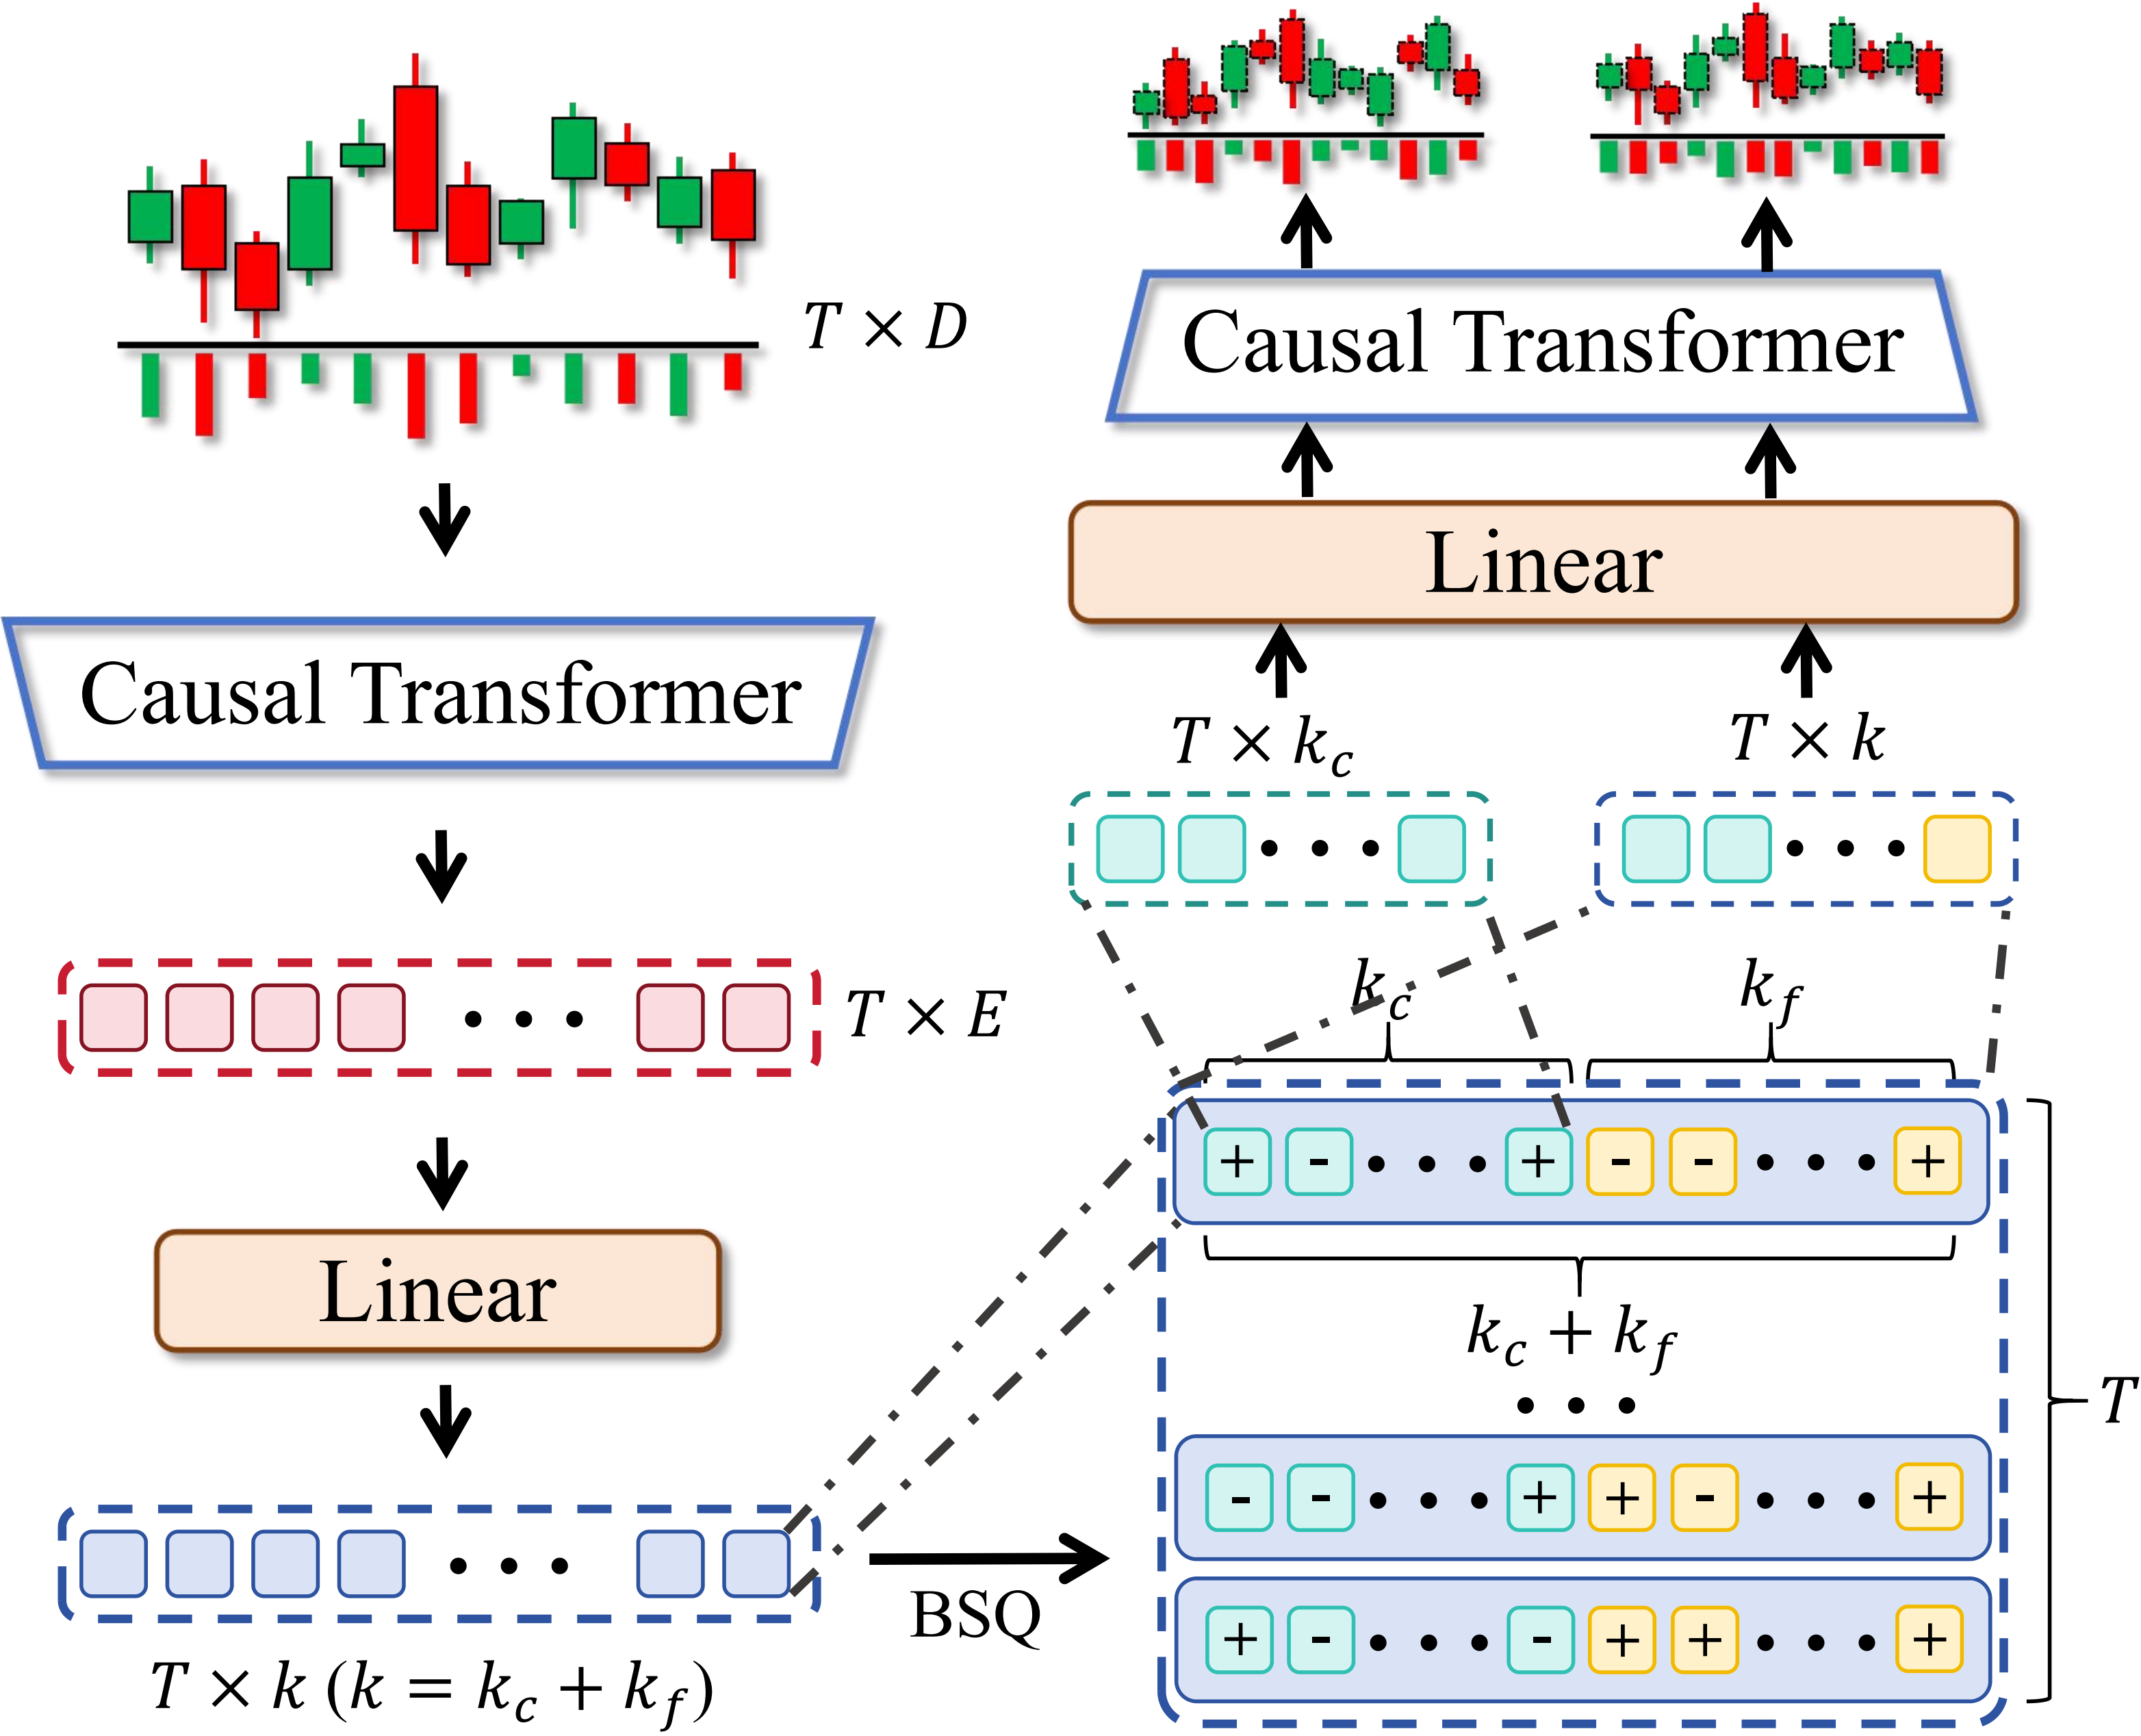
\includegraphics[width=1.0\columnwidth]{img/Tokenizer.png}
    \caption{K-line Tokenizer의 구조. 이는 Binary Spherical Quantization (BSQ) layer를 갖춘 Transformer 기반 autoencoder를 사용한다.
    % 복합 손실 목적($\mathcal{L}_{\text{coarse}}, \mathcal{L}_{\text{fine}}, \mathcal{L}_{\text{quant}}$)은 각 토큰 내부의 coarse-to-fine 표현 구조 학습을 유도한다.
    }
    \label{fig:tokenizer}
\end{figure}

\subsection{계층적 자기회귀 모델링}
\label{sec:autoregressive}

토큰화 단계 이후, 결과로 얻어진 이산 시퀀스는 $E_{\text{ar}}$로 표기되는 decoder-only Transformer를 사용해 모델링되며, 이 모델은 각 시점의 예측이 과거 문맥에만 의존하도록 causal-attention을 사용한다. 주요 목표는 토큰 시퀀스 $\mathbf{b} = \{b_1, \dots, b_T\}$에 대한 joint distribution을 추정하는 것이다. Equation~\ref{eq:ts_ar}의 단순화된 형태는 다음과 같이 유도될 수 있다:
\begin{equation}
    p(\mathbf{b}) = \prod_{t=1}^{T} p(b_t | \mathbf{b}_{<t}),
\end{equation}
여기서 $\mathbf{b}_{<t}$는 시간 $t-1$까지의 모든 이전 토큰을 나타낸다.

각 토큰이 $b_t = [b_t^{c}, b_t^{f}]$로 구조화되는 계층적 토큰 설계를 고려하여, 우리는 내재된 coarse-to-fine 의존성을 명시적으로 포착하기 위해 chain rule을 사용해 conditional probability를 추가로 분해한다:
\begin{equation}
\label{eq:chain_rule}
p(b_t | \mathbf{b}_{<t}) = p(b_t^{c} | \mathbf{b}_{<t}) \cdot p(b_t^{f} | \mathbf{b}_{<t}, b_t^{c}).
\end{equation}
이 공식화는 모델이 먼저 coarse-grained subtoken을 예측하도록 하며, 이는 이후 fine-grained residual subtoken을 생성하기 위한 scaffold 역할을 한다. 따라서 사전학습 목적은 이러한 계층적 factorization 하에서 관측된 시퀀스의 log-likelihood를 최대화하는 것으로 귀결된다.

Figure~\ref{fig:overview} (Right)에 나타난 바와 같이, 자기회귀 과정은 각 시점에 대한 통합 입력 벡터를 구성하는 것에서 시작한다. 구체적으로 시간 $i$에서 subtokens $b_i^{c}$와 $b_i^{f}$는 서로 다른 두 embedding layer를 사용해 각각 벡터 표현으로 독립적으로 투영되어, 각각 $e_c(b_i^{c})$와 $e_f(b_i^{f})$ 표현을 생성한다. 그런 다음 이러한 embeddings를 concatenate하고 선형 투영하여 융합된 입력 벡터를 생성한다:
\begin{equation}
\label{eq:embedding}
    \mathbf{v}_i = W_{\text{fuse}}([e_c(b_i^{c}); e_f(b_i^{f})]),
\end{equation}
여기서 $[\cdot;\cdot]$는 concatenation을 나타내며, $W_{\text{fuse}}$는 결합된 표현을 모델의 latent space로 투영하는 학습 가능한 weight matrix이다.

융합된 입력 시퀀스 $\{\mathbf{v}_1, \dots, \mathbf{v}_{t-1}\}$는 Transformer $E_{\text{ar}}$에 의해 처리되어 contextualized hidden states를 출력한다. $\mathbf{b}_{< t}$를 처리하여 얻은 최종 hidden state는 $\mathbf{h}_t$로 표기되며, 이후 토큰 $b_t$를 예측하는 데 사용된다. 이 hidden state는 다음 단계에서 coarse 및 fine subtokens 모두의 자기회귀 예측에 정보를 제공하여, 모델이 데이터에 내재된 multi-scale temporal dependencies를 효과적으로 포착할 수 있게 한다.

\textbf{Coarse Subtoken 예측.} History vector $\mathbf{h}_t$는 선형 head $W_c$에 의해 투영되어 첫 번째 subtoken distribution에 대한 logits를 생성한다:
\begin{equation}
    p(b_{t}^{c} | \mathbf{b}_{< t}) = \text{softmax}(W_c \mathbf{h}_t)
\end{equation}

\textbf{Fine Subtoken 예측.} Equation~(\ref{eq:chain_rule})의 conditional dependency를 모델링하기 위해, 문맥은 예측된 coarse subtoken $\hat{b}_{t}^{c}$로 업데이트되어야 한다. 학습 중에는 ground-truth subtoken(즉, teacher-forcing)을 사용하는 대신, 예측 분포 $p(b_{t}^{c} | \mathbf{b}{< t})$에서 샘플링된 이전 단계의 모델 자체 예측 $\hat{b}_{t}^{c}$를 사용한다. 우리는 이러한 샘플링 전략이 exposure bias를 완화하여 모델 견고성을 향상시키고, ground-truth tokens를 사용할 수 없는 multi-step inference의 auto-regressive 특성과 학습 분포를 더 잘 정렬한다고 본다. 우리는 $\hat{b}_{t}^{c}$의 embedding이 query로 작용하고 history $\mathbf{h}_t$가 key와 value를 제공하는 cross-attention mechanism을 사용한다. 그 결과는 두 번째 head $W_f$에 의해 투영된다:
\begin{equation}
\begin{aligned}
    \mathbf{h}^{\text{update}}_t = \text{CrossAttn}&(q=e_c(\hat{b}_{t}^{c}), k=v=\mathbf{h}_t) \\
    p(b_{t}^{f} | \mathbf{b}_{< t}, b_{t}^{c}) &= \text{softmax}(W_f \mathbf{h}^{\text{update}}_t)
\end{aligned}
\end{equation}
전체 학습 목적 $\mathcal{L}_{\text{ar}}$는 두 예측 단계에 대해 합산된 데이터의 negative log-likelihood이다:
\begin{equation}
    \mathcal{L}_{\text{ar}} = - \mathbb{E}_{\mathbf{b} \sim \mathcal{D}} \sum_{t=1}^{T} \left[ \log p(b_t^{c} | \mathbf{b}_{<t}) + \log p(b_t^{f} | \mathbf{b}_{<t}, b_t^{c}) \right]
\end{equation}
여기서 $\mathcal{D}$는 data distribution을 나타낸다.

\begin{table}[t]
\centering
\setlength{\tabcolsep}{4pt}

\resizebox{\columnwidth}{!}{%
  \begin{tabular}{l ccccc c}
  \toprule
  & 레이어 & $\mathbf{d}_{\text{model}}$ & $\mathbf{d}_{\text{ff}}$ & 헤드 & 어휘 ($2^k$) & 파라미터 \\
  \midrule
\text{Kronos}$_{small}$ & 8 & 512  & 1024 & 8 & 20 & 24.7M \\
\text{Kronos}$_{base}$  & 12 & 832 & 2048 & 16 & 20 & 102.3M \\
\text{Kronos}$_{large}$ & 18 & 1664 & 3072 & 32 & 20 & 499.2M \\
  \bottomrule
  \end{tabular}%
}
\caption{Kronos family의 model configurations. Transformer layers 수, model dimension ($\mathbf{d}_{\text{model}}$), feed-forward dimension ($\mathbf{d}_{\text{ff}}$), attention heads 수, vocabulary size, 그리고 총 parameters 수를 상세히 제시한다.}
\label{tab:kronos_configs_resized}
\end{table}

\subsection{모델 사전학습}

\begin{figure*}[t!]
    \centering
    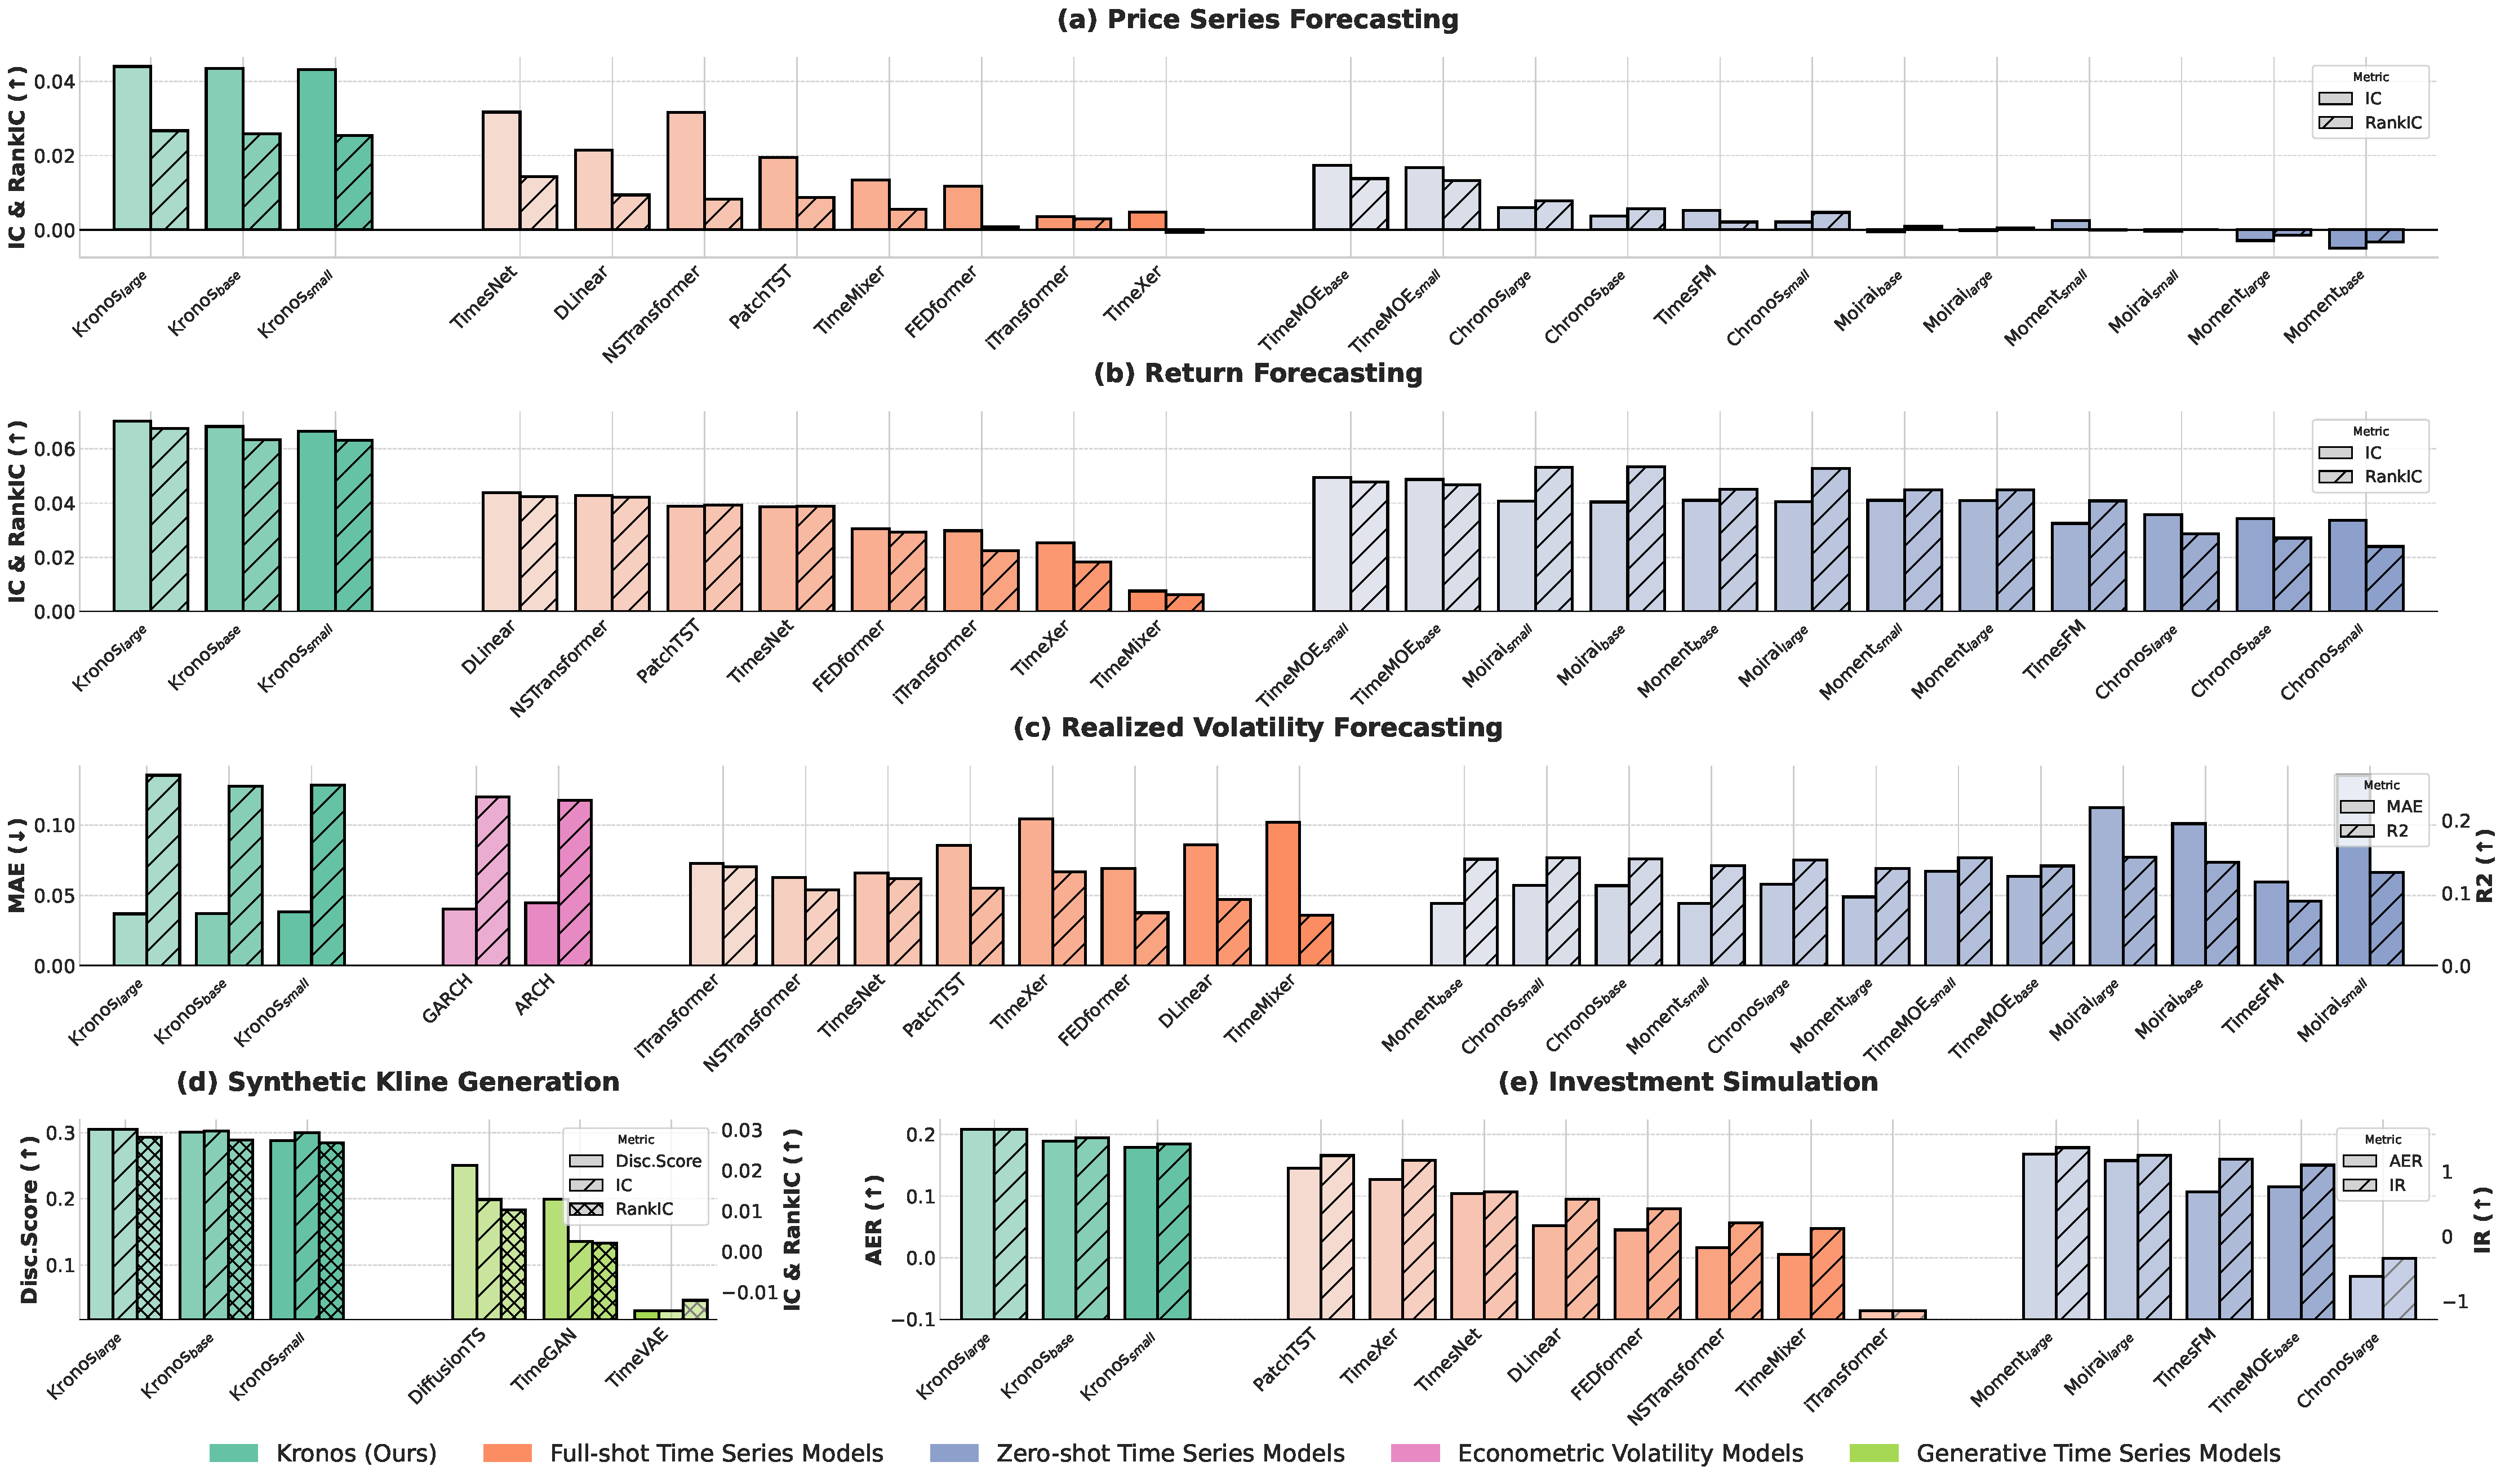
\includegraphics[width=1.0\textwidth]{img/main_result.pdf}
    \caption{다섯 가지 대표 금융 과제 전반의 주요 실험 결과. Subfigures (a-c)는 price series, returns, realized volatility에 대한 forecasting performance를 보여준다. Subfigure (d)는 fidelity와 usefulness 측면의 generative model performance를 나타낸다. Subfigure (e)는 investment simulation backtesting results를 제시한다.}
    \label{fig:main_result}
\end{figure*}

\paragraph{데이터셋}
사전학습의 품질을 보장하기 위해, 우리는 대규모 고품질 금융 K-line dataset을 처음부터 구축한다. 잘 정제된 공개 datasets를 쉽게 모을 수 있는 일반 time series에 대한 foundation-model 연구와 달리, 포괄적이고 고품질인 금융 데이터는 여전히 제한적이다. 우리의 dataset은 7개의 sampling frequencies에 걸쳐 120억 개가 넘는 observations를 포함하며, 45개 글로벌 exchanges에서 수집된 광범위한 asset classes를 포괄한다. 데이터 품질을 보장하기 위해, 우리는 금융 K-line 데이터의 고유한 특성에 맞춘 간소화된 data-cleaning pipeline을 개발하며, 이는 비정상적인 price spikes나 장기간의 inactivity와 같은 저품질 segments를 식별하고 필터링한다. Cleaning pipeline에 대한 추가 세부 사항은 Appendix~\ref{sec:dataset_details}에서 확인할 수 있다.

\paragraph{모델 학습} LLM에서 관찰된 scaling laws~\cite{kaplan2020scaling}에 근거하여, 우리는 성능과 inference budget 사이의 trade-off를 제공하기 위해 parameter count를 증가시킨 세 가지 Kronos variants를 거의 0.5 billion까지 학습했다. 자세한 model configurations는 Table~\ref{tab:kronos_configs_resized}에 제시되어 있다.
자원 제약과 실제 deployment scenarios를 고려하여, 우리는 최대 context length를 512 tokens로 제한한다. 그럼에도 이 설계는 다양한 frequencies의 K-line 데이터를 활용함으로써 임의의 forecasting horizons와 완전히 호환된다. 예를 들어, 단기 forecasting에는 1-minute data를 사용하고 weekly 또는 monthly predictions에는 daily data를 사용할 수 있다. 전체 training details는 Appendix~\ref{sec:implementation_details}에 제공된다.

\paragraph{추론} Inference 시에는 text generation과 유사하게 미래 token sequences를 자기회귀적으로 생성한다. 이 과정의 stochasticity는 temperature scaling 및 top-$p$ (nucleus) sampling~\cite{holtzman2019curious}과 같은 표준 기법을 통해 제어된다. Logits $\mathbf{z}$에서 token $i$를 샘플링할 확률은 $p_i \propto \exp(z_i / T)$로 주어지며, 여기서 $T$는 temperature이다. 높은 precision이 필요한 과제의 경우, 여러 future trajectories(즉, Monte Carlo rollouts)를 생성하고 decoded continuous values를 평균하여 더 안정적인 forecast를 생성함으로써 prediction accuracy를 향상시킬 수 있다. 우리의 실험에서 입증된 바와 같이, 이 접근법은 forecast quality를 일관되게 개선한다.
